%
\section{Semantic and Visual Clustering}
\label{sec_inhalt}

The nodes received through the tree-based search are potentially very large (i.e., many pictures were found for the node). We found a rather small semantic and a large visual diversity within these nodes. It is therefore appropriate to refine especially the large nodes into smaller clusters.

\subsection{General Approach}
Since semantics are more meaningful to humans, and thus likely to be more important for the given use case, the refinement is done first on a semantic and then on a visual basis. That is, the results from the groups with semantically similar pictures are clustered again into subclusters with visually similar pictures. The steps are explained in more detail in sections \ref{sec_keywordclustering} and \ref{sec_visualclustering}.
This approach has the additional advantage that outlier images, which have been assigned to a node but do not quite fit with the others because they show something different, can be filtered out in the semantic step. \\
The subclustering explained below and summarized in figrue \ref{fig_semanticandvisual} will only take place for nodes/clusters with a certain minimum size and results in the structure of three nested Arrays of the WordnetNode class' attribute \emph{subclusters} shown in figure \ref{fig_nodestructure}.

\begin{figure}[h]
\centering
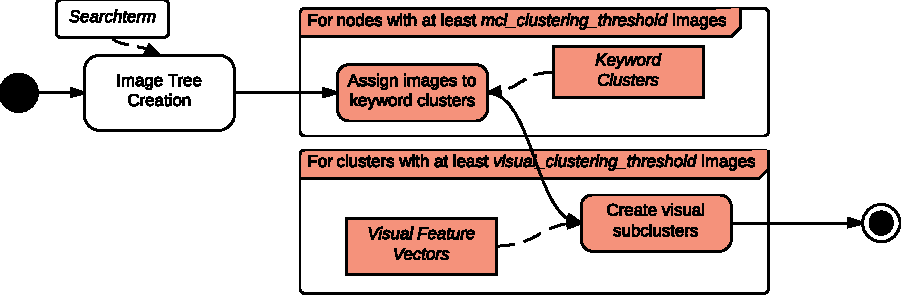
\includegraphics[width=\textwidth]{images/semantic_and_visual_clustering.pdf}
\caption{Process of Semantic and Visual Clustering}
\label{fig_semanticandvisual}
\end{figure}

The data structures used in the process, such as Image Lookup Structures and Visual Feature Vectors, need only be calculated once for each image set. The preparational processes are visualized by Figure \ref{fig_precalcprocess}.

\begin{figure}[h]
\centering
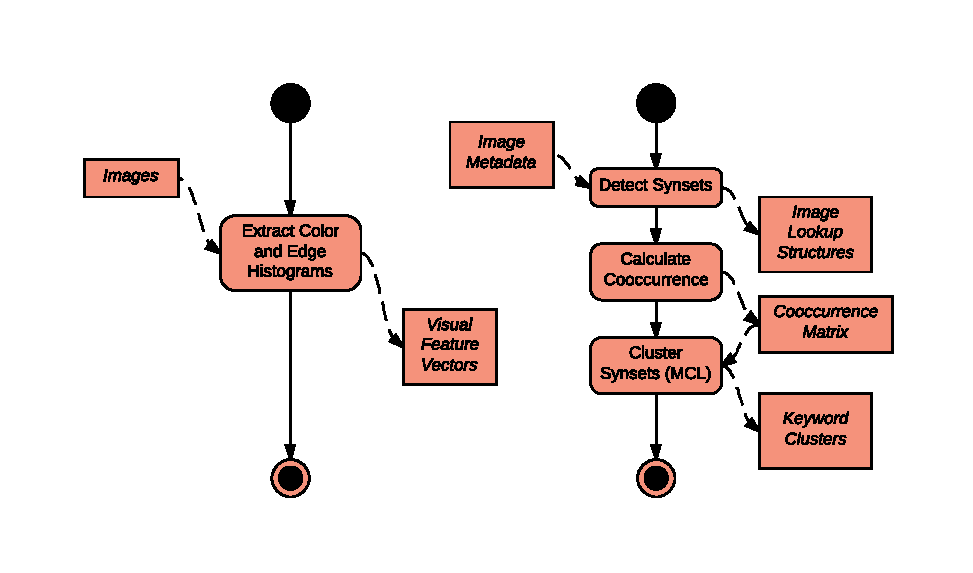
\includegraphics[width=0.8\textwidth]{images/precalcs_activity_diagram.pdf}
\caption{Static structures creation processes}
\label{fig_precalcprocess}
\end{figure}


\subsection{Keyword Clusters}
\label{sec_keywordclustering}
good for context(?), outlier identification, basic clustering for part-meronym spanned trees (Africa example)

\bigskip
Semantic clustering is accomplished by using the assigned Synsets. Therefore, Synsets are clustered into groups and pictures are assigned to these groups. According to the paper of Grigory Begelman \cite{begelman2006automated}, our first approach of clustering Synsets used co-occurrences to span a graph of related Synsets. With the help of the proposed graph clustering algorithm, it is possible to group related Synsets. But, the algorithm requires calculation of eigenvalues and eigenvectors for large sparse matrices. Furthermore, it does not take edge weighting into account.

Use MCL graph clustering algorithm\cite{Dongen1998} \todo{basic explanation of mcl algorithm}.\\
graph nodes are Synsets, edges their cooccurrence

\bigskip
for each image, count how many synsets it shares with each cluster, and assign it to maximum (can be multiple), so all images with maximum tags in that keyword cluster form one semantic cluster. Example: some parrot pictures fall into keyword cluster with persons, others in those with trees. \\
if only one image falls into a keyword cluster, consider it an outlier and remove it

\subsection{Visual Clusters}
\label{sec_visualclustering}

One difficulty in the visual part of our work, besides the choice of appropriate features and their implementation, is the question how to use them jointly in a suitable algorithm for clustering.

\subsubsection{Features}
The features we chose to use in our tool are:
\begin{itemize}
\item{Color histogram} in HSV color space with 20 bins each
\item{Edge histogram} lengths and angles, histograms with 10 bins (i.e., separation into 10 angles, with count of edges and sum of lengths for each) as combined vector \todo{make the following sound less copied}
\\
For edge histogranm extraction we use the EdgeHistogramFeatureExtractor class from the SimpleCV library. Referring to the official SimpleCV documentation \footnote{Reference: http://simplecv.sourceforge.net/doc/SimpleCV.Features.html}  the method creates histograms for the edge lengths and angles. The number of bins is used to define which and how many line directions are taken in consideration.
\end{itemize}
The reasons we chose these are that they are easy to calculate, rather obvious and humanly comprehensible. Since the purpose of this visual clustering is only in refining the semantic clusters, and not in trying to distinguish concepts by visual features, there is no apparent need for the use of more complex features. \\
\todo{Can we explain or prove that somehow?}


\subsubsection{Clustering}
A first, rather naive approach to clustering the visual characteristics extracted would be to concatenate the feature vectors (histograms), and apply one of the established clustering algorithms like k-means. \index{K-Means} The fact that remains unseen in this approach is that, generally, the values of different features are usually measured on different scales and therefore vary in their orders of magnitude: In color histogram, each bin's value represents a number of pixels, whereas in edge histograms the number of edges is counted, which is significantly smaller. \\
This circumstances influences any algorithm based on the distance between two images. Since differences in the larger values will usually be larger in its absolute value, they will also be more influential to the overall distance than the dimensions with smaller values.

So, instead, we decided to apply k-means separately for colors and edges, and join the results later through \emph{late fusion}\index{Late Fusion}, as explained below. As no specific criteria exist for the number of clusters that should be achieved, k is chosen by the established rule of thumb: $ k = \sqrt{n} $ \todo{reference to rule of thumb}, where n is the number of items to be clustered. K-means was chosen over hierarchical clustering, because it provided more well- and equally-sized clusters, the latter often just split off single images.\\
Initially, we planned to use an adaptive k, that is, start with a small k and increase it until the error (mean distance from centroids). Despite its higher computation complexity, it provides no better results than the rule of thumb. For example in color clustering, the adaptive approach will often just separate black and white images from colored ones.\\
For feature extraction, we use a pyramidal appraoch similar to the one proposed in \cite{Lazebnik2006}. Its advantage is that ... \todo{Explain advantages of pyramidal feature extraction}\\
Same paper also states the appropriateness of this method especially in refining existing clusters.\\
We combine the single-feature clusters by intersecting them, which is a simple and performant late fusion method \index{Late Fusion}. It ensures that all images within a cluster are similar in color as well as edge structure and leads to less or equal to $ 2\sqrt{k} $ subclusters.
